% !TEX TS-program = xelatex
% !TEX encoding = UTF-8 Unicode
% !Mode:: "TeX:UTF-8"

\documentclass{resume}
\usepackage{zh_CN-Adobefonts_external} % Simplified Chinese Support using external fonts (./fonts/zh_CN-Adobe/)
%\usepackage{zh_CN-Adobefonts_internal} % Simplified Chinese Support using system fonts
\usepackage{linespacing_fix} % disable extra space before next section
\usepackage{cite}
\usepackage{textpos}
\usepackage{xcolor}
\usepackage{tcolorbox}
\usepackage{graphicx,calc}
\newlength\myheight
\newlength\mydepth
\settototalheight\myheight{Xygp}
\settodepth\mydepth{Xygp}
\setlength\fboxsep{0pt}
\definecolor{tumblue}{HTML}{0065BD}
\begin{document}
\pagenumbering{gobble} % suppress displaying page number

\name{温柄辉}

% {E-mail}{mobilephone}{homepage}
% be careful of _ in emaill address
\contactInfo{(+86) 189-1626-6067}{wbhwenbinghui@gmail.com}{}{}
% {E-mail}{mobilephone}
% keep the last empty braces!
%\contactInfo{xxx@yuanbin.me}{(+86) 131-221-87xxx}{}
 
\newcommand{\UniversitaetLogoBreite}{19mm}
\newcommand{\SeitenrandOben}{1cm}
\begin{textblock*}{\UniversitaetLogoBreite}[1,0](\textwidth-10mm, -2.0cm)%
	\raggedleft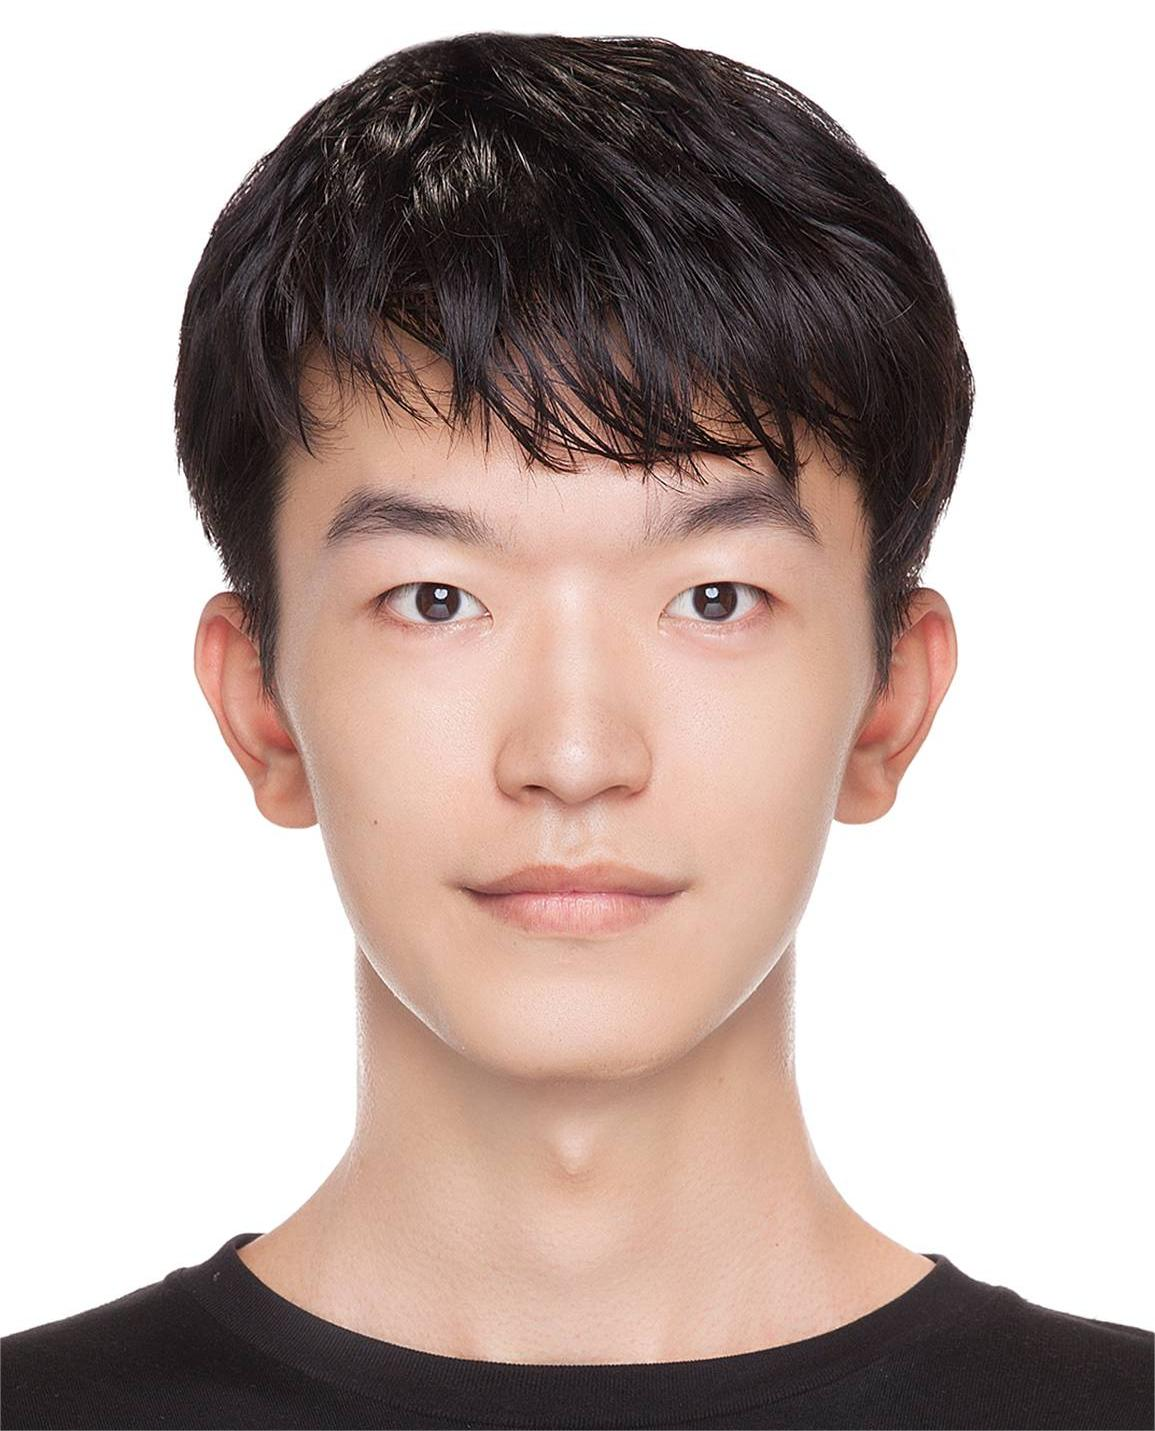
\includegraphics[width=0.85in]{我的照片_裁剪.jpg}%
\end{textblock*}
 
\section{个人总结}
\begin{itemize}
\item {自学能力强,勤奋好学;愿意抓住机会,渴望提高自己的能力}
\item {有丰富的编程实现及开发感知检测,场景重建,视觉SLAM,点云相关等算法经验(包括经典算法以及深度学习)}
\item {掌握C++, Python (深度学习了解pytorch,以及mmcv框架), Matlab等编程语言,Git版本管理以及多线程/分布式应用开发}
\item {英语,德语水平胜任文献阅读以及日常会话}
\end{itemize}

% \section{\faGraduationCap\ 教育背景}
\section{教育背景}
\datedsubsection{\textbf{慕尼黑工业大学(\textcolor{tumblue}{QS排名37}), \textit{硕士研究生} }}{2021.10 - 至今}
\datedsubsection{预计2023年12月毕业; 计算机学院: 机器人感知与人工智能}{德国慕尼黑} 
\datedsubsection{\textbf{同济大学}, \textit{工学学士}}{2016.8 - 2021.7}
\datedsubsection{汽车学院: 车辆工程}{上海} 

% \section{\faCogs\ IT 技能}
%\section{技术能力}
%% increase linespacing [parsep=0.5ex]
%\begin{itemize}[parsep=0.2ex]
%  \item \textbf{编程语言}: JavaScript (ECMAScript, Node.js), HTML/CSS, Python, Go, SQL, C, Shell
%  \item \textbf{操作系统,数据库与工程构建}: Linux/macOS/MySQL/MongoDB/Git/webpack/Progressive Web App
%  \item \textbf{关键词}: React/Vue.js/D3.js(SVG)/three.js(canvas, WebGL)/chrome extension/Express
%\end{itemize}

% \end{itemize}
\section{论文发表}
\textbf{Binghui Wen$^*$, Haoang Li$^*$, Ming Gao$^*$, Jinhu Dong$^*$} "Semantic Scene Completion via Deformable Deep Implicit Templates", \textbf{ICCV 2023} 顶级计算机视觉会议已接收
\begin{itemize}
	\item 提出新算法,新思路, 使用深度学习进行场景重建 [3D场景点云$\Rightarrow$3D 实例网格], 效果优于目前同问题Sota (RfD-Net, DIMR)结果(论文多半代码由我编写)
\end{itemize}
\section{项目与实习经历}
\datedsubsection{\textbf{\raisebox{0mm}{{
\includegraphics[height=\myheight]{Momenta_Logo.png}}}}\ 感知部门建图定位算法实习生}{2023.4-至今}
\begin{itemize}
  \item 建图定位组算法实习生,主要工作为\textcolor{tumblue}{\textbf{建图与定位}}相关算法的创新改进以及应用等,算法包含传统多视角几何以及深度学习
\end{itemize}
\datedsubsection{\textbf{Multi-Module Fusion BEV Map Prediction}, 毕业设计项目}{2023.5-至今}
\begin{itemize}
  \item 深度关联多种输入模态信息,深度信息监督视觉特征,视觉语义增广点云特征;可选模态包括视觉,LiDAR,以及HD map; 
  \item 旨在实现\textcolor{tumblue}{\textbf{深度学习端到端}}精准预测自动驾驶场景鸟瞰语义分割地图,并帮助高精定位校正误差
\end{itemize}

\datedsubsection{\textbf{Camera Localization in 3D LiDAR Maps}}{2022.10-2023.1}
\begin{itemize}
  \item 运用已有大型点云,在视觉SLAM算法中实现实现相机定位 (ORB-SLAM框架, C++, Ceres, Pangolin, PCL, TBB并行); 锻炼了C++编写中型
  项目的能力,以及改进算法实现程序高效运行的能力
\end{itemize}


\datedsubsection{\textbf{Mixed-Integer-Programming-based Motion Planner}}{2022.4-2022.10}
\begin{itemize}
	\item 使用混合整数优化方法规划自动驾驶车辆运动轨迹 (Python, Gurobi, Cplex); 规划控制,独立建立数学模型并检验算法,对带约束最小二乘线性优化问题建模以及优化有一定了解
\end{itemize}

\datedsubsection{\textbf{蔚来\ \raisebox{0mm}{{
\includegraphics[height=4.6mm]{NIO_logo.svg.png}}}}\ 自动驾驶系统实习生}{2021.7-2021.10}
\begin{itemize}
	\item 参与自动驾驶数据平台的建立,主要工作为车端试验信息切片、算法还原、数据归纳等部分代码编写; 锻炼了合作编程开发能力
\end{itemize}

\datedsubsection{\textbf{国家大学生创新性实验计划项目: 中心城区大型居住小区停车问题解决方案}}{2018.9-2019.9}
\begin{itemize}
	\item 通过充分的准备和优秀的表现,在校内的答辩中脱颖而出,进入国家级大学生创新性实验计划项目比赛,并凭借此项目获得创新创业论坛三等
	奖;准备和进行项目展示/报告的经验充分
	\item 参加 “互联网+” 大学生创新创业大赛并且获得银奖
\end{itemize}


\section{社团和组织经历}
\datedsubsection{\textbf{DIAN Racing同济电车队 底盘转向组}}{ }
\begin{itemize}
	\item 成员 底盘部转向组,参与转向系统的设计以及制造
\end{itemize}
\datedsubsection{\textbf{同济大学汽车文化宣讲团外联部}}{ }
\begin{itemize}
	\item 成员 参加同济汽车文化宣讲团,曾在上海多所中小学宣讲汽车文化;喜欢汽车文化,愿意上台分享
\end{itemize}

\section{技能/证书及其他}
% increase linespacing [parsep=0.5ex]
\begin{itemize}[parsep=0.2ex]
  \item \textbf{技能:} C++, Python, Matlab, Git, Linux操作, SSH
  \item \textbf{语言:} 英语(CET-6,雅思) 德语 (C2, Test Daf 5444)
  \item \textbf{兴趣爱好:} 编程,学习前沿科技,电子游戏,Wargame
\end{itemize}


% \section{\faHeartO\ 项目/作品摘要}
% \section{项目/作品摘要}
% \datedline{\textit{An Integrated Version of Security Monitor Vis System}, https://hijiangtao.github.io/ss-vis-component/ }{}
% \datedline{\textit{Dark-Tech}, https://github.com/hijiangtao/dark-tech/ }{}
% \datedline{\textit{融合社交网络数据挖掘的电视节目可视化分析系统}, https://hijiangtao.github.io/variety-show-hot-spot-vis/}{}
% \datedline{\textit{LeetCodeOJ Solutions}, https://github.com/hijiangtao/LeetCodeOJ}{}
% \datedline{\textit{Info-Vis}, https://github.com/ISCAS-VIS/infovis-ucas}{}


%% \section{\faInfo\ 社会实践/其他}
%\section{社区参与/实践其他}
%% increase linespacing [parsep=0.5ex]
%\begin{itemize}[parsep=0.2ex]
%  \item 乐于参与开源社区讨论,\textbf{参与翻译 Vue.js, webpack, WebAssembly, Babel 文档,印记中文成员}
%  \item 中国科学院大学2016秋季学期可视化与可视分析课程助教,\textit{http://vis.ios.ac.cn/infovis-ucas/}
%  \item 未来论坛学生会成员、北理社联新闻信息中心主任、北理工软件学院学生会宣传部副部长(2012-2016)
%  \item 2013-2015 北京市共青团“温暖衣冬”志愿者,第九届园博会志愿者,2014 FLL机器人世锦赛志愿者
%\end{itemize}NIO_logo.svg.png

%% Reference
%\newpage
%\bibliographystyle{IEEETran}
%\bibliography{mycite}
\end{document}
